\documentclass[12pt]{article}
\usepackage[utf8]{inputenc}
% Greek-specific commands
\usepackage[greek,english]{babel}
\usepackage{alphabeta}

\usepackage{graphicx} % Allows you to insert figures
\usepackage{amsmath} % Allows you to do equations
\usepackage{fancyhdr} % Formats the header
\usepackage{geometry} % Formats the paper size, orientation, and margins
\usepackage{csquotes}
\usepackage{minted}
\usepackage{color}
\usepackage{hyperref} 

\hypersetup{
    pdfnewwindow=true,
    colorlinks=true,
    linkcolor=black,
    filecolor=black,      
    urlcolor=black
    }
\linespread{1.25} % About 1.5 spacing in Word
\setlength{\parindent}{0pt} % No paragraph indents
\setlength{\parskip}{1em} % Paragraphs separated by one line
\renewcommand{\headrulewidth}{0pt} % Removes line in header
\geometry{legalpaper, portrait, margin=1in}
\setlength{\headheight}{14.49998pt}

\definecolor{dkgreen}{rgb}{0,0.6,0}
\definecolor{gray}{rgb}{0.5,0.5,0.5}
\definecolor{mauve}{rgb}{0.58,0,0.82}

\begin{document}
\begin{titlepage}
    \begin{center}
         \vspace*{5cm}
 
         \Huge{Εργασία HW-2}
         
        
         \vspace{3cm}
         \large{Τζατζίδης Αντώνης}
    
         \vspace{1cm}
         \large{ΑΕΜ:9938}
        
        \vfill
     \end{center}
\end{titlepage}

\section*{Σύνοψη}
Σκοπός της εργασίας ήταν η σχεδίαση και προσομοίωση 2 κυκλωμάτων, ενός FIFO και ενός counter στη SystemVerilog  μαζί με κάποια 
assertions που μας δώθηκαν καθώς και από ενα testbench στο καθένα για τη βεβαίωση της σωστής λειτουργίας του κυκλώματος.

\section*{Counter Module}
Για τη σχεδίαση χρησιμοποίησα μία εσωτερική μεταβλητή που "μαζεύει" τα 3 σήματα που καθορίζουν την λειτουργία του μετρητή 
(ld\_cnt,count\_enb,updn\_cnt), η οποία ανανεώνεται σε ένα always\_comb block.
\begin{minted}[escapeinside=||,mathescape=true,frame=single,framesep=10pt]{SystemVerilog} 
logic [2:0] state_info;
|$\dots$|
always_comb begin : set_state
    state_info = {ld_cnt,count_enb,updn_cnt};
end 
\end{minted}

Το always\_ff block ενεργοποιείται στη θετική ακμή του ρολογιού ή στην αρνητική του rst αφού λειτουργεί ασύγχρονα. 
Αν δεν είναι ενεργοποιημένο το rst
τότε ο μετρητής ανανεώνει την τιμή του με βάση την μεταβλητή state\_info. Χρησιμοποίησα priority case ώστε να τηρείται η προτεραιότητα
μεταξύ των 3 σημάτων όπως αναφέρονται στις οδηγίες. 
\begin{minted}[escapeinside=||,mathescape=true,frame=single,framesep=10pt]{SystemVerilog} 
always_ff @ (posedge clk, negedge rst) 
begin
    if(!rst) data_out <= 16'b0;
    else 
    begin
        priority case(state_info) 
            3'b 000: data_out <= data_in;
            3'b 001: data_out <= data_in;
            3'b 010: data_out <= data_in;
            3'b 011: data_out <= data_in;
            3'b 100: data_out <= data_out; 
            3'b 101: data_out <= data_out; 
            3'b 110: data_out <= data_out - 1;
            3'b 111: data_out <= data_out + 1;
        endcase
    end
end
\end{minted}
\section*{Counter Assertions}
Τα assertions έχουν ίδια δομή όπως στο παράδειγμα. Mε τη χρήση του ifdef επιλέγουμε ποιό θέλουμε να ενεργοποιήσουμε ώστε να είναι
πιο εύκολος ο έλεγχος τους. Το πρώτο assertion ελέγχει αν η έξοδος είναι 0 στη θετική ακμή του ρολογιού 
όταν ενεργοποιείται το reset.
\begin{minted}[escapeinside=< >,mathescape=true,frame=single,framesep=10pt]{SystemVerilog} 
`ifdef reset
property pr1;
    @(negedge prst) 1'b1  |-> @(posedge pclk) pdata_out == 16'd0;
endproperty
\end{minted}
Το δεύτερο ελέγχει αν η έξοδος παραμένει σταθερή όταν ενεργοποιούμε το pcount\_enb (και το rst δεν είναι ενεργό) 
χρησιμοποιώντας το \$stable.
\begin{minted}[escapeinside=< >,mathescape=true,frame=single,framesep=10pt,breaklines]{SystemVerilog} 
`elsif count_stable
property pr2;
    @(posedge pclk) disable iff(!prst) (pld_cnt && !pcount_enb) |-> @(negedge pclk) $stable(pdata_out);
endproperty
\end{minted}
To τρίτο ελέγχει αν τα υπόλοιπα 2 σήματα που καθορίζουν την έξοδο έχουν τις κατάλληλες τιμές (και το rst δεν είναι ενεργό)
ανάλογα με την τιμή του updn\_cnt ο μετρητής αυξάνει ή μειώνει την έξοδο κατά 1. Επειδή το δεξί μέρος του assertion ελέγχεται
στην αρνητική ακμή του ρολογιού θέλουμε την τιμή του updn\_cnt στον προηγούμενο κύκλο καθώς τότε καθορίζεται αν θα αυξηθεί η θα μειωθεί
το data\_out γι' αυτό χρησιμοποίησα το \$past(pupdn\_cnt).
\begin{minted}[escapeinside=< >,mathescape=true,frame=single,framesep=10pt,breaklines]{SystemVerilog} 
`elsif count_updown                   
property pr3;
    @(posedge pclk) disable iff(!prst) (pld_cnt && pcount_enb) |-> @(negedge pclk) ($past(pupdn_cnt)) ? (pdata_out == $past(pdata_out) + 16'd1) : (pdata_out == $past(pdata_out) - 16'd1);
endproperty
\end{minted}
\section*{Counter Testbench}
Το testbench ακολουθεί τη δομή του παραδείγματος και δοκιμάζει διάφορες περιπτώσεις που κάνουν trigger τα assertions.
\begin{figure}
\vspace*{-1cm}
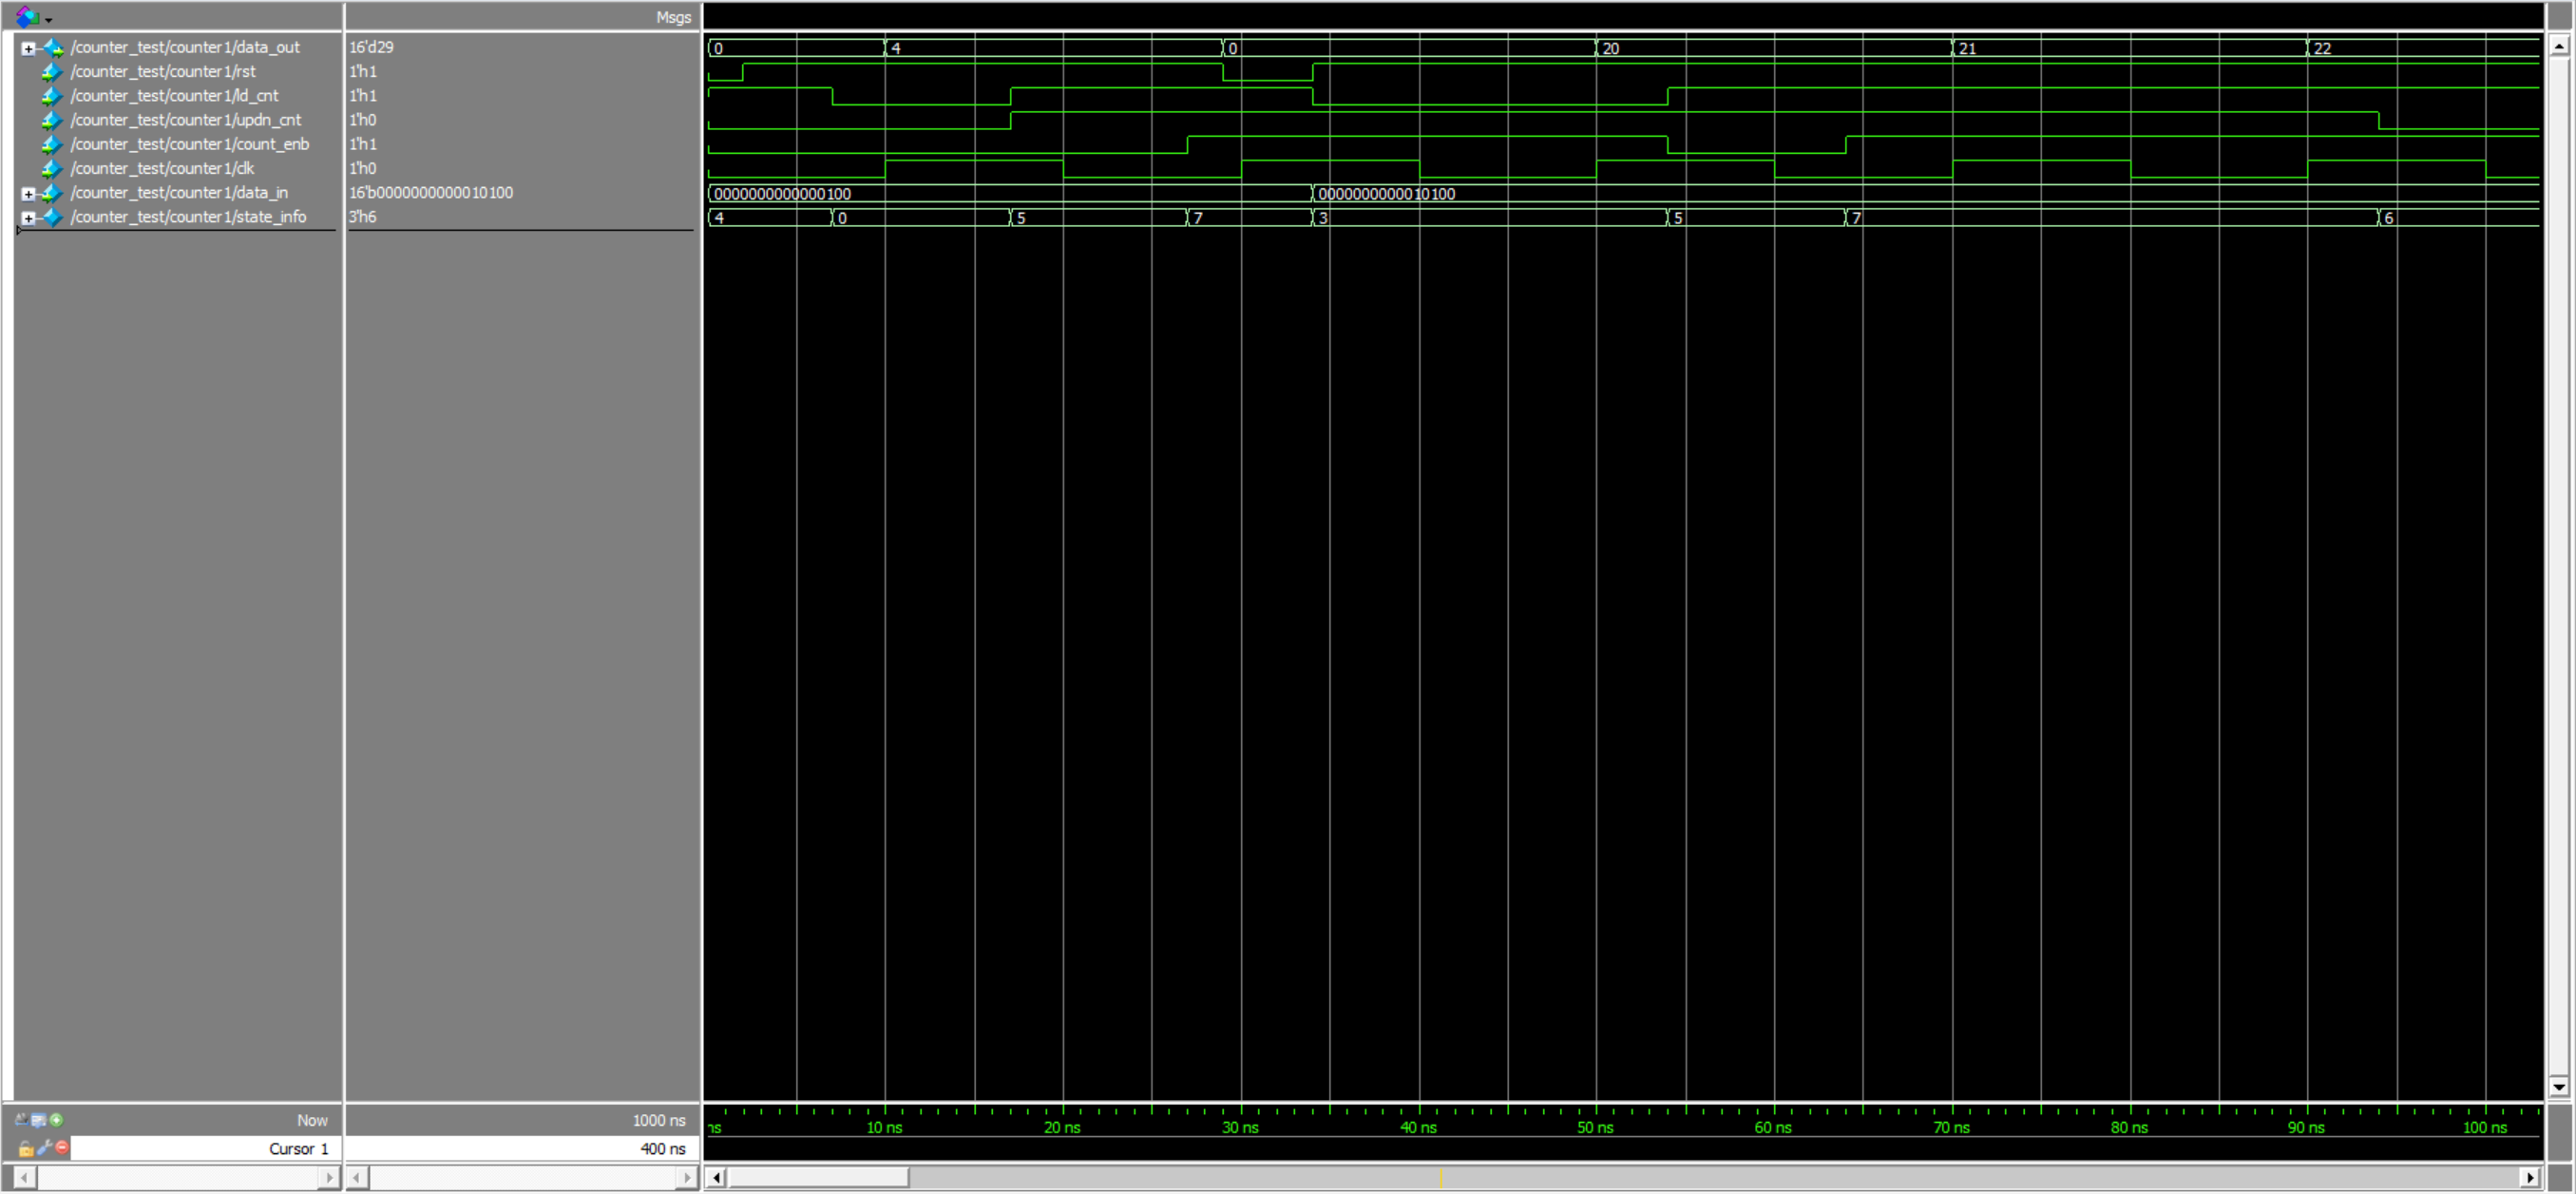
\includegraphics[width=\textwidth,height=.7\textheight,keepaspectratio]{counter_1.png} 
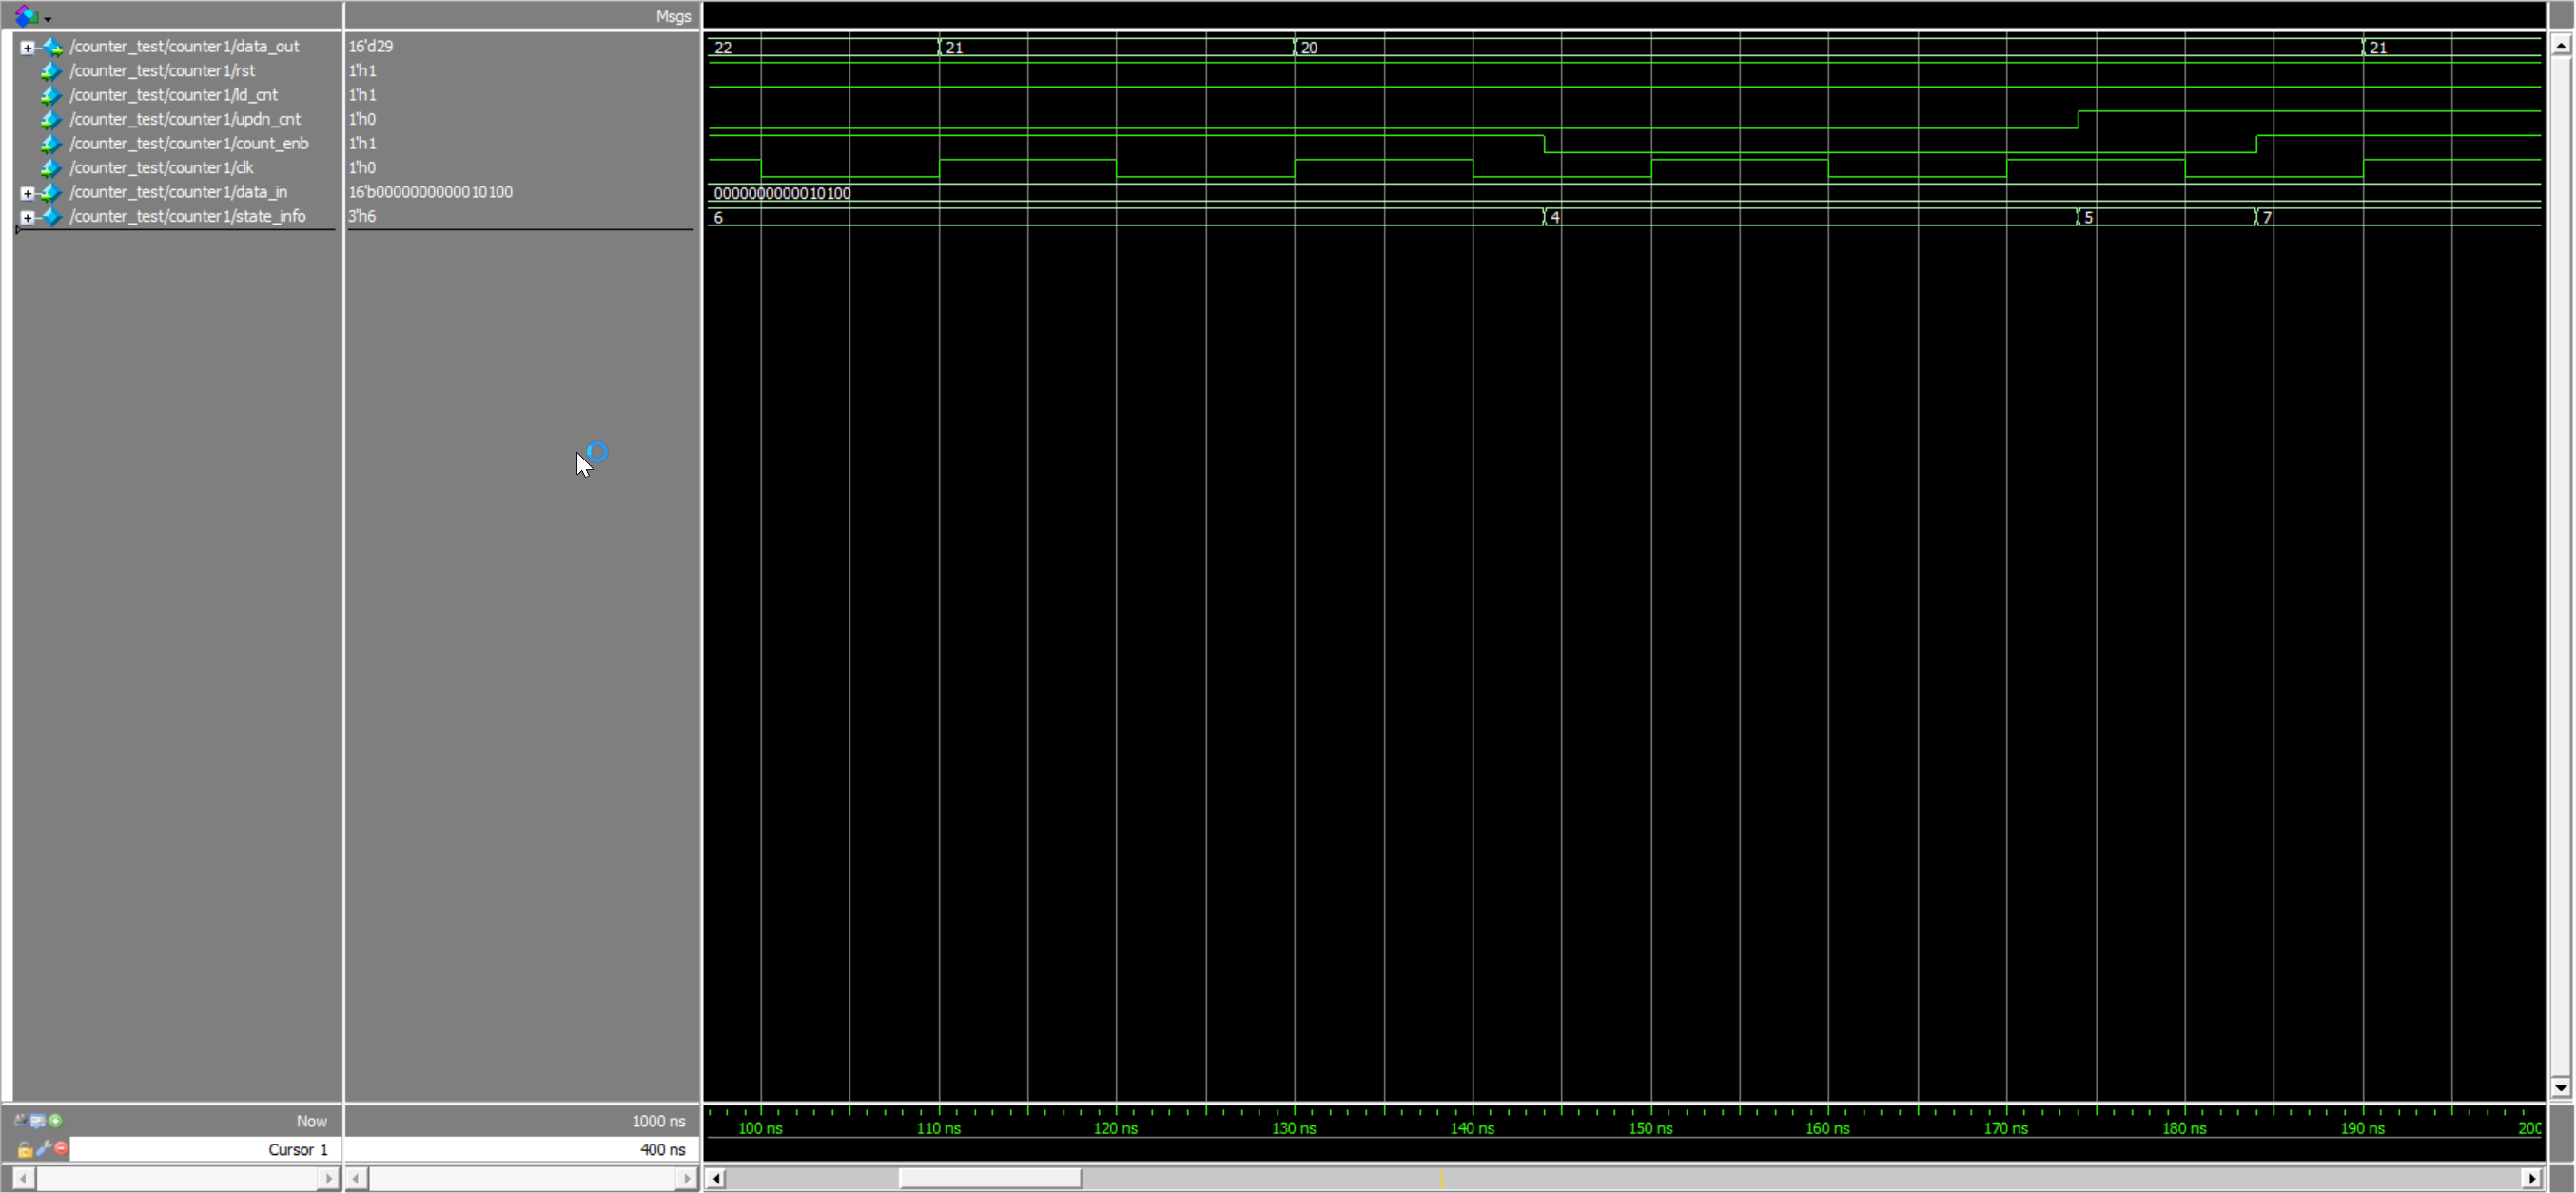
\includegraphics[width=\textwidth,height=.7\textheight,keepaspectratio]{counter_2.png}
\end{figure}
\section*{FIFO Module}
Το FIFO δέχεται δύο παραμέτρους: DATA\_WIDTH και FIFO\_DEPTH οι οποίες έχουν default τιμές 16. Για τον υπολογισμό
των bits που απαιτούνται για τα τους write και read pointers χρησιμοποίητει η μέθοδος \$clog2 ώστε να έχουν
$log_2$ FIFO\_DEPTH bits. Επειδή ο counter μπορεί να
γίνει ίσος με το FIFO\_DEPTH προσθέτουμε ένα έξτρα bit για να μην έχουμε overflow. Επιπλέον όπως πριν το state\_info
"μαζεύει" τα σήματα fifo\_write, fifo\_read. Τέλος το regs είναι ένα array μήκους FIFO\_DEPTH και κάθε στοιχείο
αποτελείται από DATA\_WIDTH bits, σ'αυτό θα αποθηκεύονται και θα διαβάζονται τα δεδομένα. 
\begin{minted}[escapeinside=||,mathescape=true,frame=single,framesep=10pt]{SystemVerilog} 
logic [$clog2(FIFO_DEPTH)-1:0] wr_ptr,rd_ptr;
logic [$clog2(FIFO_DEPTH):0] cnt;
logic [DATA_WIDTH-1:0] regs [0:FIFO_DEPTH-1];
logic [1:0] state_info;
\end{minted}

To state\_info και το ασύγχρονο reset λειτουργούν όπως στο προηγούμενο κύκλωμα. Αν το reset δεν είναι ενεργό, στη θετική
ακμή του ρολογιού διακρίνονται 3 περιπτώσεις ανάλογα με τα σήματα read και write (αν κανένα από τα 2 δεν είναι ενεργό, τότε
το FIFO δεν κάνει τίποτα). 
\begin{itemize}
\item Αν και τα 2 σήματα είναι ενεργά τότε ελέγχει αν το FIFO είναι γεμάτο για να διαβάσει πριν γράψει, 
διαφορετικά πρώτα διαβάζει και μετά γράφει, αυξάνει τους write και read pointers (το cnt δεν αλλάζει αφού έχουμε μια ανάγνωση και μία εγγραφή) 
και ελέγχει με βάση τη συνθήκη που δώθηκε αν είναι γεμάτο η άδειο.
\item Αν μόνο το fifo\_read είναι ενεργό ελέγχει πρώτα αν το FIFO είναι άδειο. Αν δεν είναι διαβάζει, αυξάνει το read\_ptr,
μειώνει το cnt και ελέγχει αν είναι άδειο (προφανώς δεν μπορεί να είναι γεμάτο). Επειδή οι εντολές θα εκτελεστούν ταυτόγχρονα
ο έλεγχος για το αν είναι άδειο θα γίνει με το cnt$-$1.
\item Το αντίστοιχο συμβαίνει αν μόνο το fifo\_write είναι ενεργό. 
\end{itemize} 
\begin{minted}[escapeinside=< >,mathescape=true,frame=single,framesep=10pt,breaklines]{SystemVerilog} 
case(state_info)
    2'b11: begin
            if(cnt >= FIFO_DEPTH)
            begin
                fifo_data_out <= regs[rd_ptr];
                regs[wr_ptr] <= fifo_data_in;
                rd_ptr <= rd_ptr + 1;
                wr_ptr <= wr_ptr + 1;
                
            end
            else
            begin
                regs[wr_ptr] <= fifo_data_in;
                fifo_data_out <= regs[rd_ptr];
                wr_ptr <= wr_ptr + 1;
                rd_ptr <= rd_ptr + 1;
            end
            fifo_empty <= (cnt == 0) ? 1:0;
            fifo_full  <=  (cnt >= FIFO_DEPTH) ? 1:0;


    end
    2'b01: begin
            if(cnt == 0) fifo_empty <= 1;
            else 
            begin
                fifo_data_out <= regs[rd_ptr];
                rd_ptr <= rd_ptr + 1;
                cnt <= cnt - 1;
                fifo_empty <= (cnt-1 == 0) ? 1:0;
                fifo_full <= 0;
            end
            
    end 
    2'b10: begin
            if(cnt >= FIFO_DEPTH) fifo_full  <= 1;
            else
            begin
                regs[wr_ptr] <= fifo_data_in;
                wr_ptr <= wr_ptr + 1;
                cnt <= cnt + 1;
                fifo_full  <=  (cnt+1 >= FIFO_DEPTH) ? 1:0;
                fifo_empty <= 0;
            end
    end
    default: continue;
endcase
\end{minted}
\section*{FIFO Assertions}
Τα assertions χρησιμοποιούν εκτός από τα inputs και outputs του module τα εσωτερικά σήματα read\_pointer, write\_pointer και cnt.
 Χωρίζονται σε 3 ομάδες με τα ifdef όπως στο προηγούμενο παράδειγμα. 
\begin{itemize}
\item Στην πρώτη ελέγχεται η λειτουργία του reset όπως στον counter.  
\begin{minted}[escapeinside=< >,mathescape=true,frame=single,framesep=10pt,breaklines]{SystemVerilog}
`ifdef reset
property pr1;
    @(negedge prst) 1'b1  |-> @(posedge pclk) (!pfifo_full && pfifo_empty && pcnt == 0);
endproperty
\end{minted}
\item Στην δεύτερη ελέγχεται αν λειτουργούν σωστά οι συνθήκες για τα output fifo\_full, fifo\_empty    
\begin{minted}[escapeinside=< >,mathescape=true,frame=single,framesep=10pt,breaklines]{SystemVerilog} 
`elsif empty_full
property pr1;
    @(posedge pclk) disable iff(!prst) pcnt == 0 |-> pfifo_empty == 1;
endproperty

property pr2;
    @(posedge pclk) disable iff(!prst) pcnt >= FIFO_DEPTH |->  pfifo_full == 1;
endproperty
\end{minted}
\item Στην τρίτη ελέγχεται αν το κύκλωμα δεν επιτρέπει τις εγγραφές σε γεμάτο FIFO και τις αναγώσεις σε άδειο 
βλέποντας αν ο write\_ptr ή ο read\_ptr αντίστοιχα δεν μεταβάλλεται.
\begin{minted}[escapeinside=< >,mathescape=true,frame=single,framesep=10pt,breaklines]{SystemVerilog} 
`elsif read_write_invalid
property pr1;
    @(posedge pclk) disable iff(!prst) ((pcnt >= FIFO_DEPTH) && pfifo_write && !pfifo_read) |-> @(negedge pclk) $stable(pwr_ptr);
endproperty

property pr2;
   @(posedge pclk) disable iff(!prst)  ((pcnt == 0) && !pfifo_write && pfifo_read) |-> @(negedge pclk) $stable(prd_ptr);
endproperty
\end{minted}
\end{itemize}
\section*{FIFO Testbench}
Το testbench έχει ίδια δομή με πριν με τη διαφορά ότι όταν γίνεται bind το module με τα assertions πρέπει να περαστούν και τα εσωτερικά 
σήματα cnt, write\_pointer και read\_pointer στα assertions.
\begin{minted}[escapeinside=< >,mathescape=true,frame=single,framesep=10pt,breaklines]{SystemVerilog} 
bind fifo fifo_property #(16,16) fifobound (.prst(rst), .pfifo_write(fifo_write), .pfifo_read(fifo_read), .pclk(clk), .pfifo_full(fifo_full), .pfifo_empty(fifo_empty), .pfifo_data_in(fifo_data_in), .pfifo_data_out(fifo_data_out), .pcnt(fifo.cnt), .pwr_ptr(fifo.wr_ptr), .prd_ptr(fifo.rd_ptr));
\end{minted}
Όπως και στο προηγούμενο tb, ελέγχεται η λειτουργία του FIFO δοκιμάζοντας εγγραφές και αναγνώσεις (ταυτόγχρονα και μη) 
καθώς και άκυρες εγγραφές και αναγνώσεις για να βεβαιωθεί η λειτουργία των assertions.  

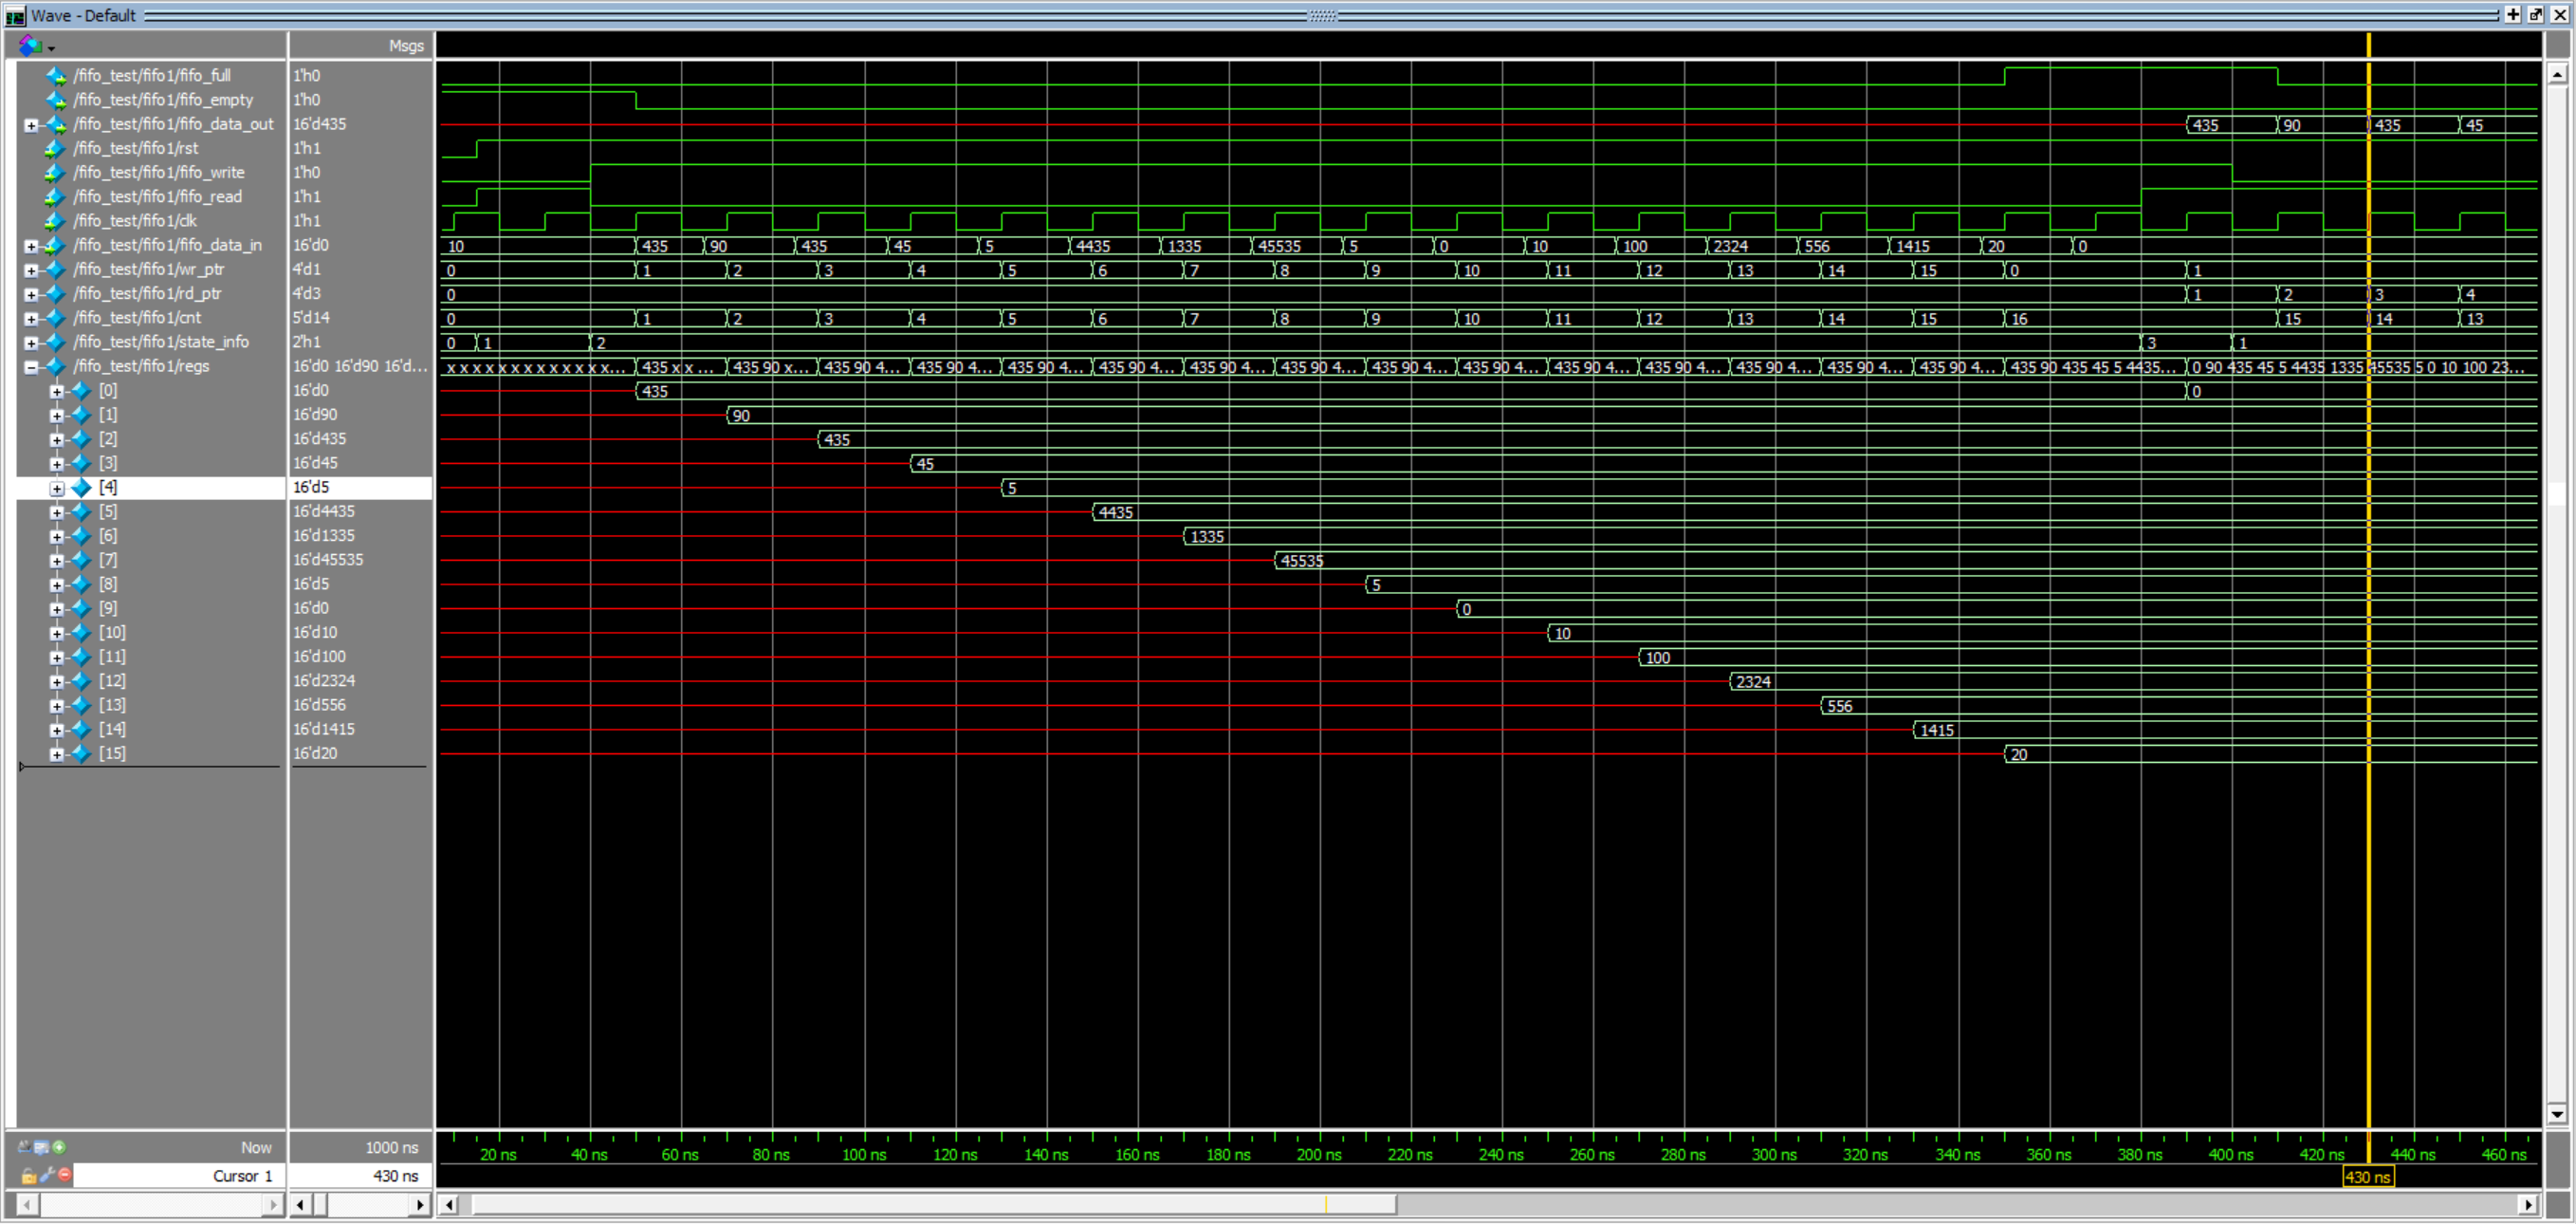
\includegraphics[width=\textwidth,height=\textheight,keepaspectratio]{fifo_1.png} 
\linebreak
\linebreak
\linebreak

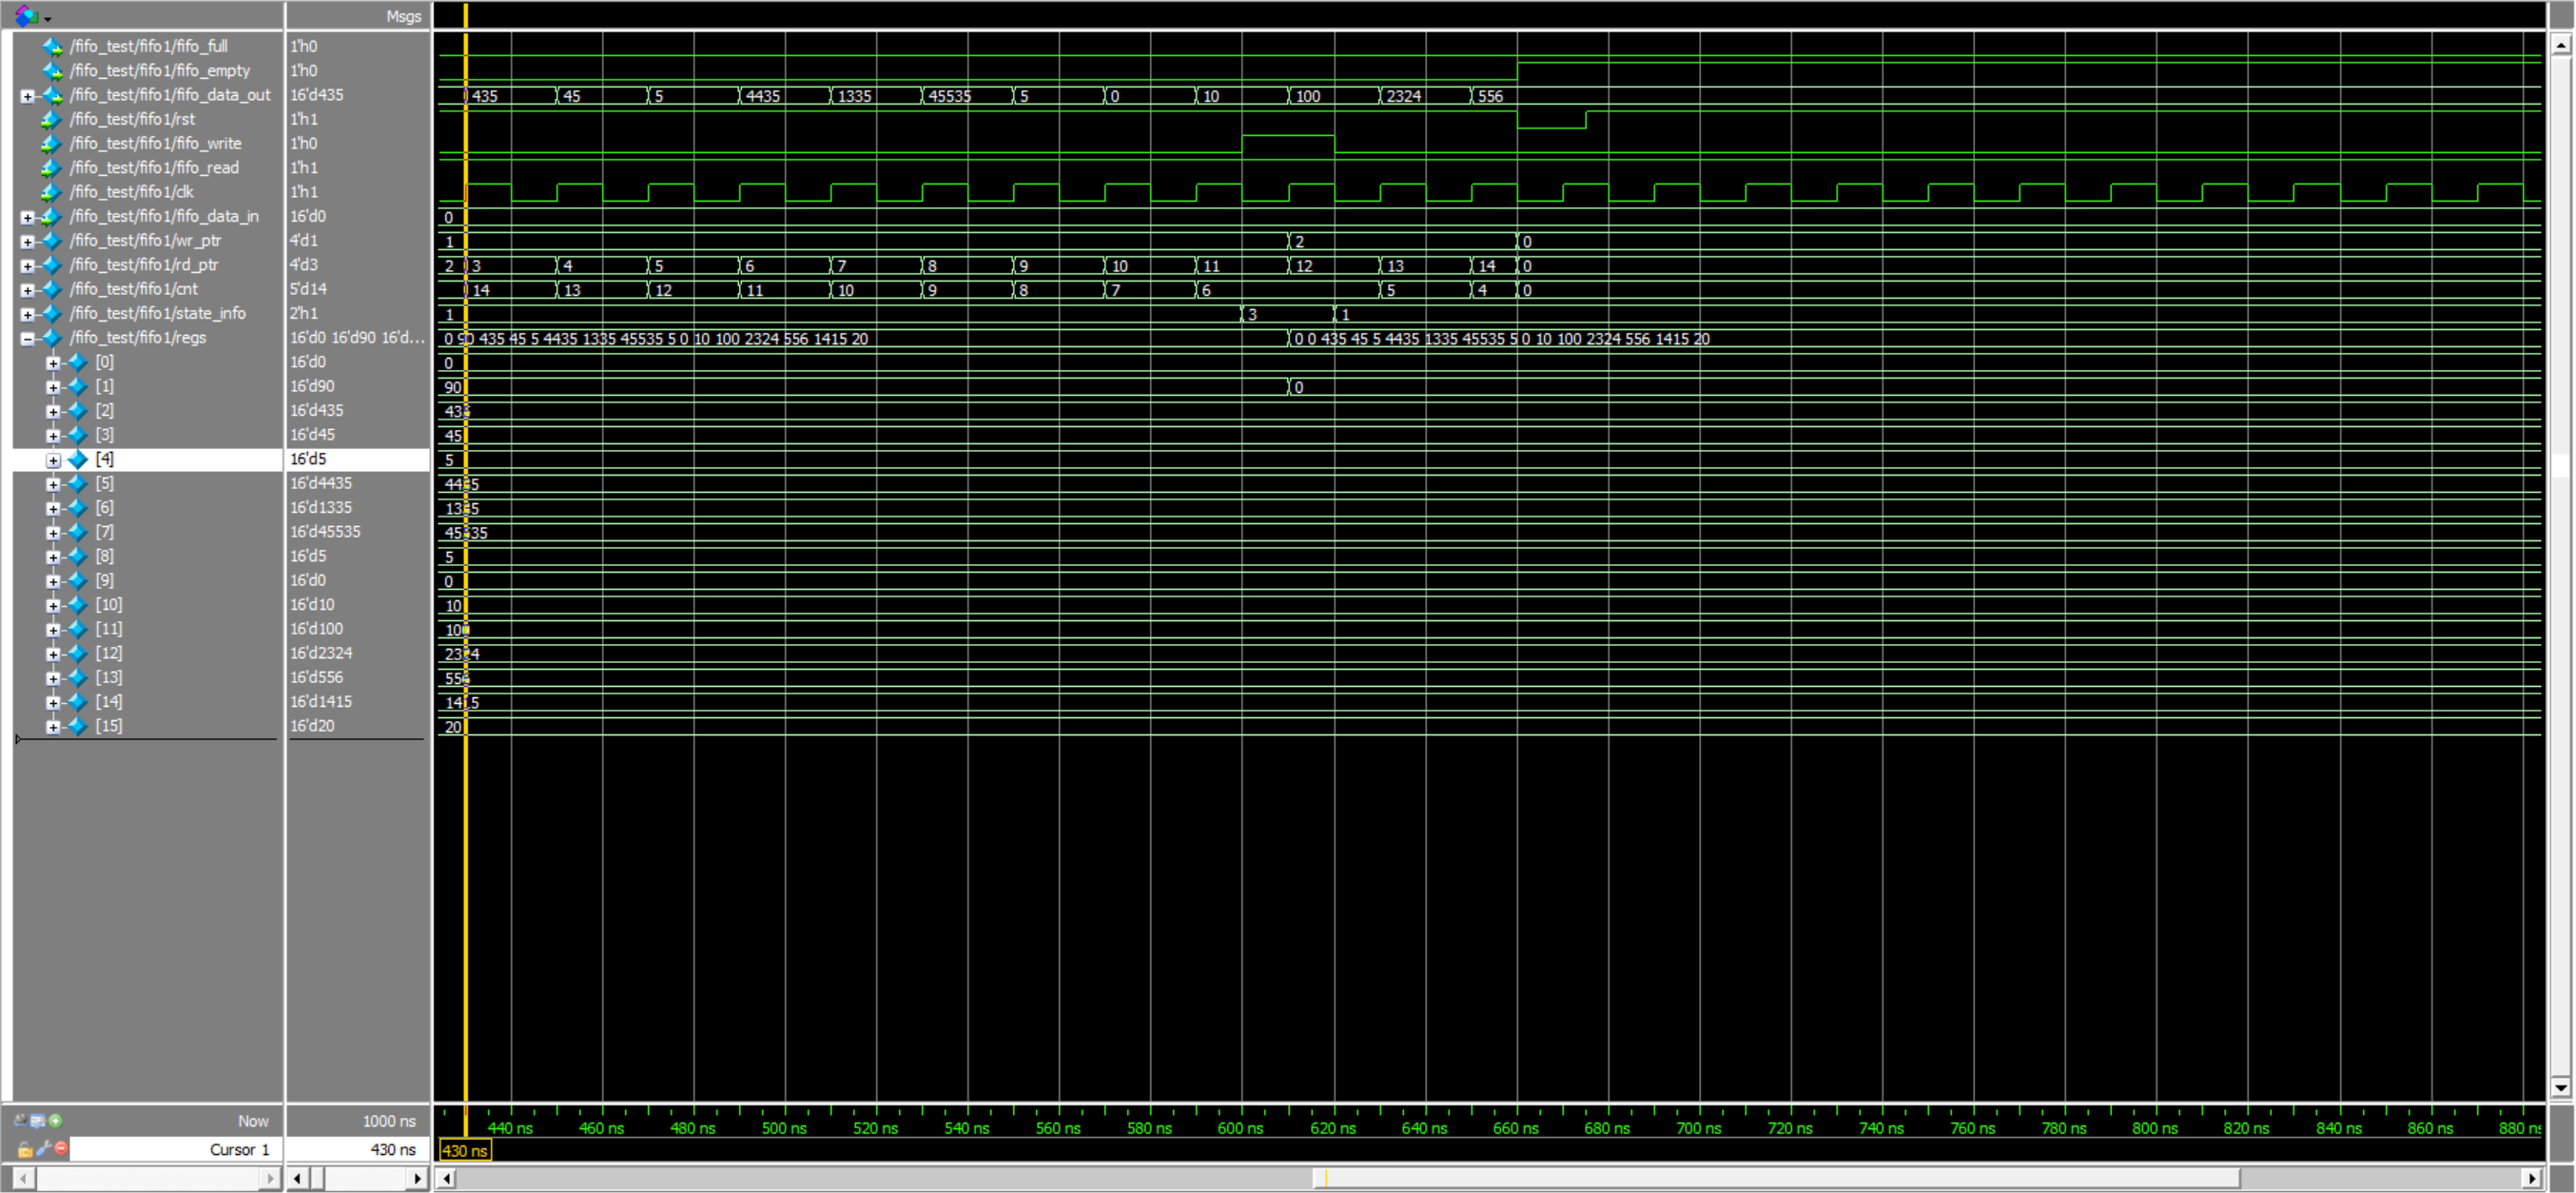
\includegraphics[width=\textwidth,height=\textheight,keepaspectratio]{fifo_2.png}

\end{document}